


\documentclass[11pt]{article}

% options 
\setlength{\oddsidemargin}{13pt}
\setlength{\evensidemargin}{13pt}
\setlength{\textwidth}{436pt}
\setlength{\textheight}{610pt}
\setlength{\voffset}{-30pt}


% packages
\usepackage{lipsum}
\usepackage{graphicx}

% macros
\usepackage{amsmath, amsfonts}
\usepackage{enumerate}

\newcommand{\Jey}{\mathcal{J}}
\newcommand{\Bee}{\mathcal{B}}
\newcommand{\Emm}{\mathcal{M}}
\newcommand{\Eff}{\mathcal{F}}
\newcommand{\Ess}{\mathcal{S}}
\newcommand{\Ell}{\mathcal{L}}
\newcommand{\reals}{\mathbb{R}}
\newcommand{\integers}{\mathbb{N}}
\newcommand{\Salg}{$\sigma$-algebra }
\newcommand{\bfP}{{\bf P}}
\newcommand{\EXP}{\text{ {\bf E}}}
\newcommand{\VAR}{\text{ {\bf Var}}}
\newcommand{\COV}{\text{ {\bf Cov}}}
\newcommand{\IND}[1]{{\bf 1}_{#1}}
\newcommand{\absv}[1]{\left| #1 \right|}


\title{Estimating Fugitive Lead Emissions: \\ Preliminary 
Results and Discussion }
\author{Bamdad Hosseini}
\date{\today}



\begin{document}

\maketitle

\begin{abstract}
  This is a short report on progress of the internship project with 
Teck resources operation in Trail, British Columbia, Canada. The project
aims towards estimating fugitive lead emissions from the Trail site 
for the period of August 20 to September 19, 2013. This report presents 
discussions on the nature of the problem and the methods that are being 
used as well as preliminary results and future challenges.
\end{abstract}

\pagebreak

\section{Introduction}
This document presents a report on the progress of an internship project 
with the Teck resources operation in Trail, British Columbia, Canada during 
the fall of 2013. The project is based on a similar project that was done 
with the same company regarding zinc emissions from a different part of the 
industrial site \cite{stockie2010inverse}. Here we aim to estimate the 
rate of fugitive emissions of lead particulates from the whole industrial 
site from various measurements of the contaminant concentration rates at 
certain times as well as monthly deposition of lead particulates due to 
gravitational settling.\\ 

 Emissions from stacks, exhausts and bag houses 
are closely monitored by the company and estimates of their emission rates 
are trusted. The issue is that measurements of lead deposition and concentrations
indicate more emissions than expected from  the known sources and 
this hints towards fugitive emissions from buildings and piles of 
products at the site. Of course it is not feasible or even informative to 
consider all possible sources of emissions such as all windows, outlets or 
roads, therefore we split the site into a number of distinct areas
and estimate all emissions from that area with a point source at the center 
of that section. This assumption allows the use of the Gaussian plume model
\cite{stockie2011siam} which greatly reduces the computational cost and makes 
the problem solvable on the order of an hour on a personal computer.\\

This report is structured as follows: In section 2 we discuss the various types 
of available data and the type of assumptions they imply. Section 3 summarizes 
the underlying assumptions of the project to this point. Section 4 is dedicated 
to preliminary results regarding total deposition of the sources and Section 5
describes what we hope to achieve in the remaining time of the project.

\section{Available data}
One of the strong points of this project is the variety  of the available types 
of data. The company has provided two main types of data; there are monthly 
accumulative deposition measurements at 30 dust-fall jars spread out through 
the industrial site and parts of the city of Trail. These are plastic 
cylindrical jars that are deployed for the period of this study and 
measure total particulate deposition through the month. In contrast 
to the dust-fall jars we also have averaged measurements of the 
 contaminant concentration from Xact, TSP and PM10 devices. The Xact equipment 
takes measurements every hour through the whole month and the TSP and PM10
equipments take 24 hour averages on selected days. Data is available from 
one Xact equipment, two TSPs and Three PM10s.\\

Looking at the time scales of these measurements we notice an issue with 
the time scales of the problem. For example, the dust-fall jars 
take monthly accumulated measurements of the particulates. These sensors 
are insensitive to instantaneous variations of wind or the source emission rates. 
They are only useful in estimating the total emissions in a month 
but not at all informative about hourly variations of the emissions. Similarly,
the TSP and PM10 are good for estimation of the emission rates during a day 
but their data cannot be trusted for shorter time scales or the periods when 
they are turned off. The Xact instrument is of course the most useful for 
estimating the emission rates on shorter time scales but then there is 
only one of these equipments available which is far from being sufficient
 for a conclusive result. With this discussion in mind we suggest that the 
best way to utilize the current data is to use all available data 
at once. This choice increases the cost of the solution and complicates 
the algorithm in many ways but these difficulties are manageable by the 
right choice of the data structure and time scales.
 
\section{Assumptions}
Before we present some preliminary results, it is 
worthwhile to summarize the underlying assumptions of the model and identify 
possible sources of uncertainty that are introduced by the simplified model.
\subsection{General setup}
\begin{itemize}
\item One of the major assumptions of the model is the constant wind velocity 
through the domain at each time interval. The wind data is available at 10 minute 
intervals at a single measurement post 
and we take this measurement to be exact and 
neglect variations of the wind on time intervals of less than 10 minutes.
\item We assume that the atmosphere is categorized as the 'C' stability class 
(slightly unstable) throughout the month. This is a compromise due to 
lack of meteorological data to make a conclusive decision. Also the 'C'
class corresponds to sunny weather with little clouds or rain which 
is the dominant weather type in the month of August in Trail. 
\item Topological variations are neglected and the domain of the problem 
is taken to be completely flat with all sensors positioned at the ground.
\item We assume the contaminant transport reaches a steady state in each 
time interval of simulations (every 10 minutes). This assumption is not 
accurate at short time 
intervals but it allows us to use the Gaussian plume model. 
\end{itemize}
\subsection{Contaminant}
\begin{itemize}
\item Only dry deposition is being considered in this model and durations of 
rain are neglected.
\item Following the dust-fall particulate characterization report \cite{EnvDustfallParticle} by the Technology group ART, we assume the contaminant is mostly 
present in the form of Pb-oxide. Material properties such as density and 
molar mass of the contaminant is taken to be constant and equal to those 
of Pbo. 
\item Based on the finding in \cite{EnvDustfallParticle} 
We take the particle size to be 5 $\mu m$ which corresponds to the 
most common particle size during the tests. This size determines the 
settling and deposition velocity of the particles. 
\item We also take the particles to be spherical so that Stoke's law 
can be used to compute the settling velocity.
\end{itemize}
\subsection{Sources}
\begin{itemize}
\item The site is split into 12 areas and emissions from all sources 
within each area is approximated by a single point source in the 
middle of that area.
\item As a compromise, all point sources are taken to be at 5 meters 
above ground as an average of height of possible sources.
\item For the purpose of this report we assume constant annual emission 
rates for all sources. This is a reasonable assumption since the 
dust-fall jars are more accurate when it comes to estimating constant emission 
rates or overall emissions.
\end{itemize}
\section{Preliminary results}
Here we present some of our preliminary findings. It is important to 
emphasize that here we only use the dust-fall measurements and 
other data types such as the Xact or PM10 data are left for the 
future. 30 dust-fall jars were deployed for the period of August 20 to 
September 19, 2013 and 28 of these receptors had useful measurements. 
We assume the dust-fall jars have a large error margin of $\pm 30 \% $
so the error is taken to be multiplicative. Solution of the inverse problem
for constant emission rates on dust-fall jars is very cheap therefore 
to estimate the effect of this measurement error we take 500 realizations 
of the data with the given uniform  $\pm 30 \%$ variation and solve the 
inverse problem for each realization. This allows us to compute the 
standard deviation of the emission rates which corresponds to an error bound 
on the estimated rates. We compute the emission rate of each source 
for the period of the month of measurements and then extrapolate this value 
to get an estimate of the annual emissions in units of tons per year. 
\\

Figure 1 shows the estimated emission rates of each area along with 
their computed error bounds. It is clear that the Smelter North 
Centroid area and the Flats North area are the major contributors to 
the emissions. The Ferrous Granules area barely any contribution to 
the emissions and its has been almost zero through the simulations. 
Using these results we estimate that a total of $28.4 \pm 1.4 \: [tn/yr]$
of lead is being emitted from the entire site. Figure 2 shows percentage of 
contributions coming from each area of the site.

\begin{figure}[htp]
  \centering
  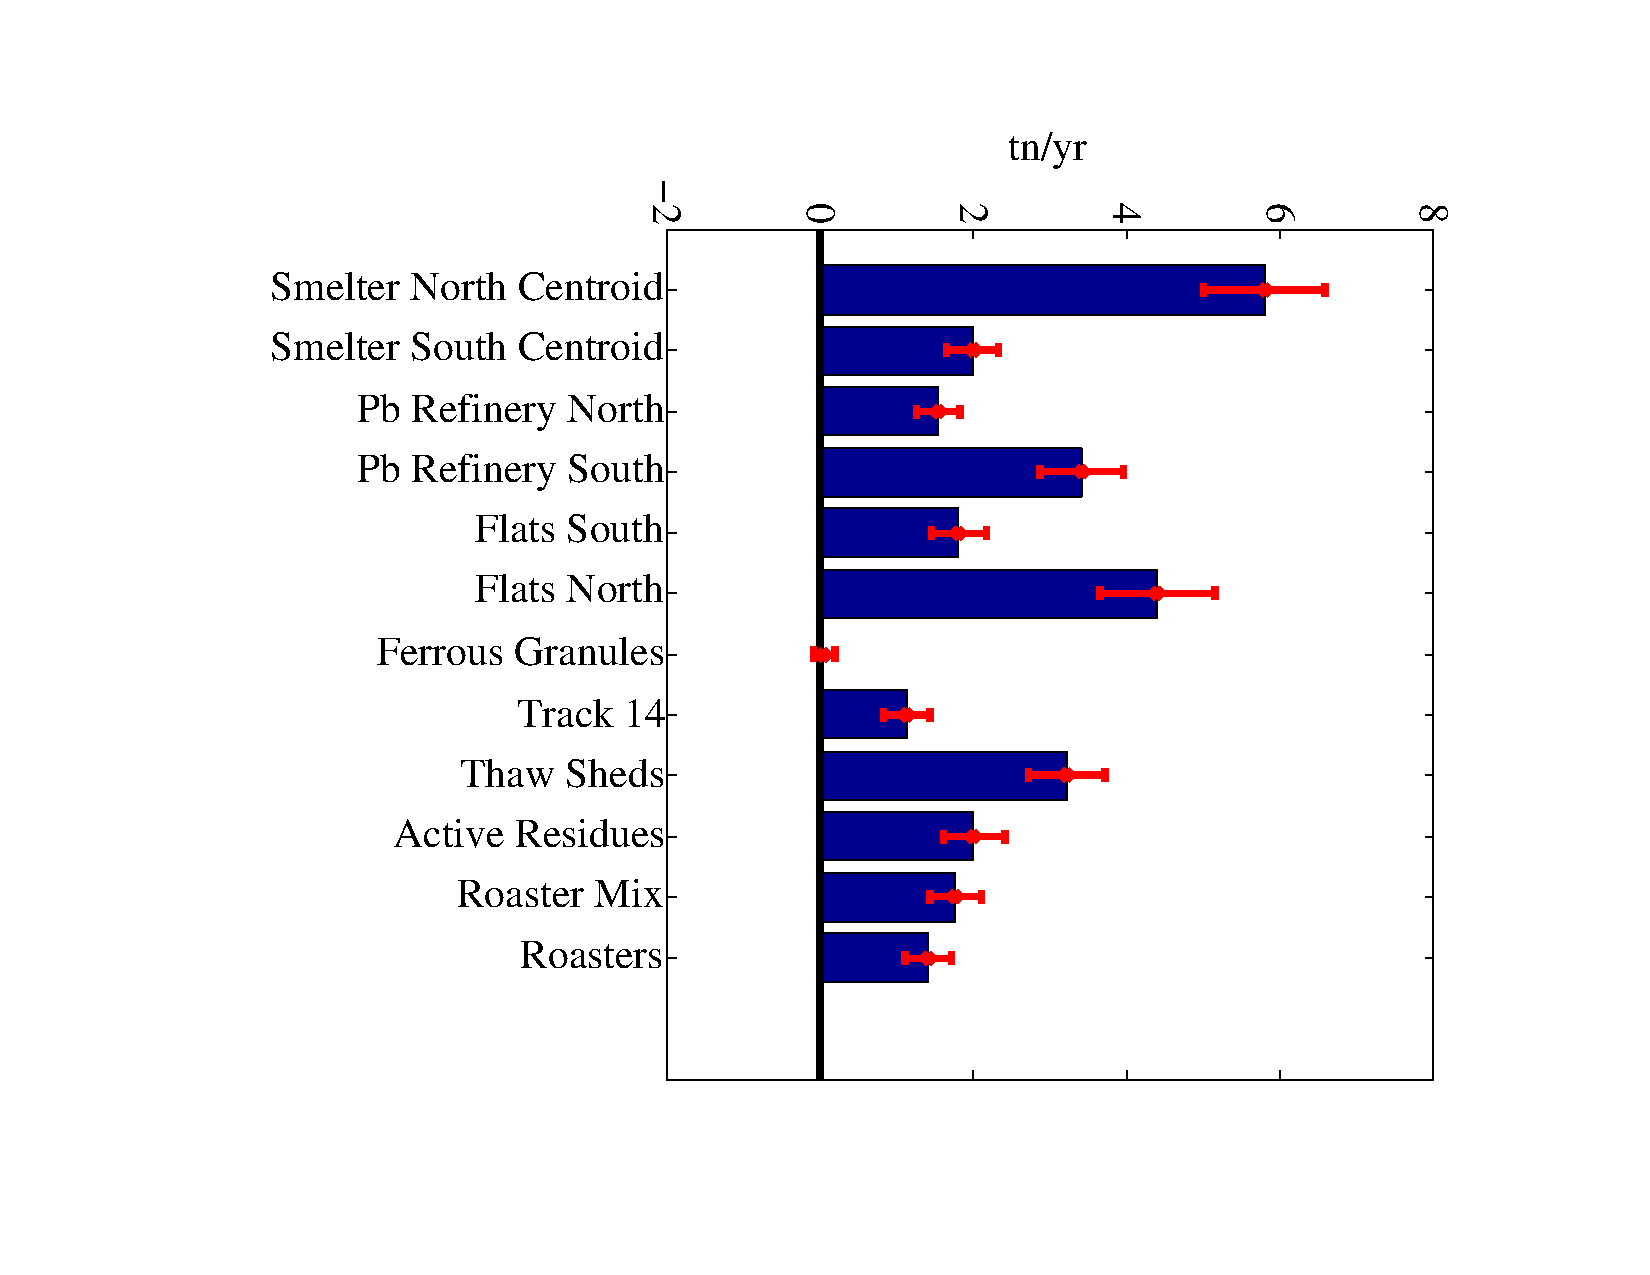
\includegraphics[angle = 90, scale = 0.5, clip = true, 
   trim = 4cm 2cm 3cm 2cm]{emissions.pdf}
  \caption{Annual emission rates of sources.}
\end{figure}

\begin{figure}[htp]
  \centering
  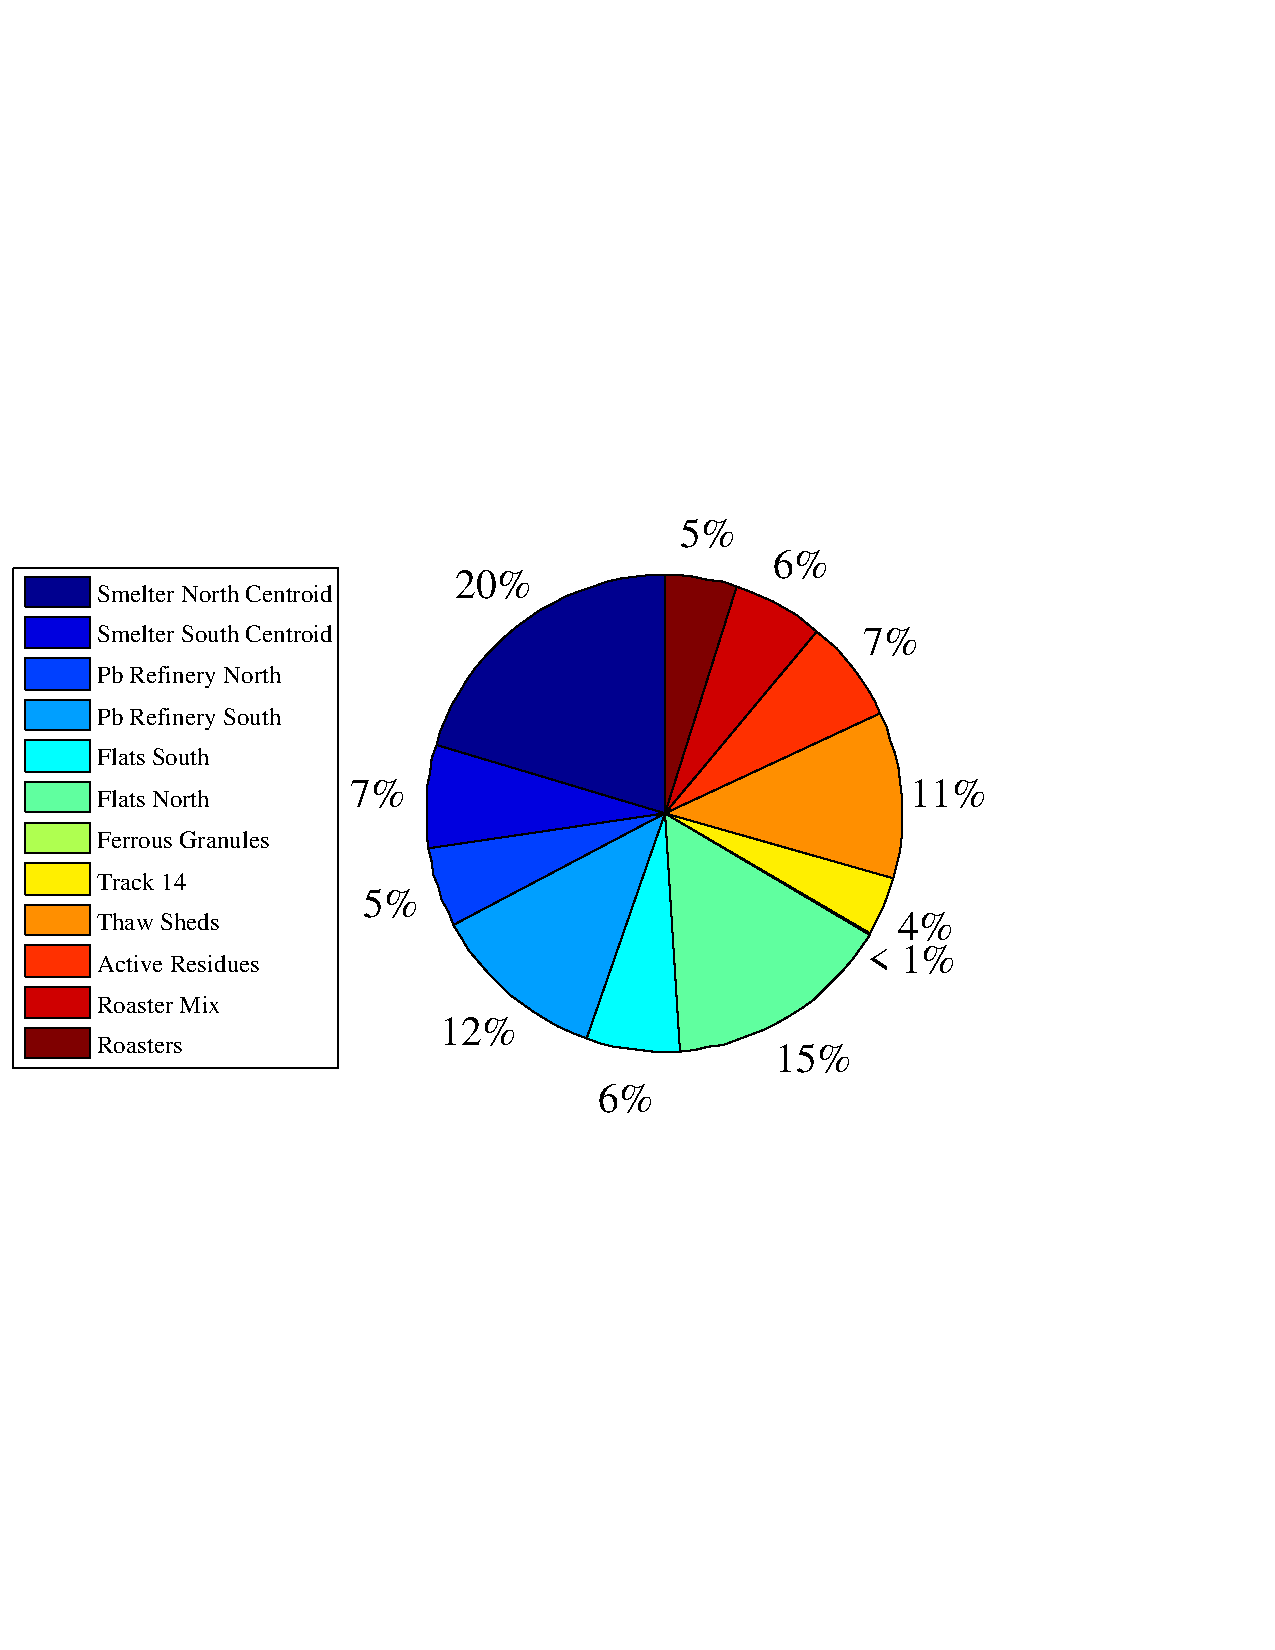
\includegraphics[angle = 0, scale = 0.7, clip = true, 
   trim = 0cm 9cm 5cm 8cm]{piechart.pdf}
  \caption{Relative contribution of sources to the total emissions.}
\end{figure}

\section{Future Work}
The main drawback of our current results is that they are based solely on 
the dust-fall jar measurements. These are useful for estimating total 
emission rates but do not contain much information regarding transient 
behavior of the sources. Also, the other available data 
types are more accurate as compared to the dust-fall jars so as explained 
in Section 2, the best approach here is to use all available data at 
once. Another restrictive assumption in our computations is the 
assumption of constant emission rates. This is not a valid assumption 
since there is more activity on the site during day shifts and many 
sources such as the roads may be completely inactive during night shifts.
With these considerations we can summarize our future goals as follows:
\begin{itemize}
\item Solve the inverse problem of emission rates with time dependent 
sources. 
\item Provide a new algorithm capable of handling all data types 
at once, this can be formulated as a multi-objective optimization 
problem to minimize misfit of all data.
\item Introduce trust weight or data quality for a more reliable
estimation. Some of the dust-fall jars are placed very close to 
unrelated sources such as roads and piles of material. These measurements 
are accompanied by large error which in turn increases uncertainty of 
results.
\item Enable the algorithm to use more of our intuitive information.
For example, we know that emissions from certain areas should be larger 
during the day shift. 
\end{itemize}

%% Copyright 1998 Pepe Kubon
%%

%% `bibl.tex' --- bibliography for thes-full.tex, thes-short-tex from
%%                the `csthesis' bundle
%%
%% You are allowed to distribute this file together with all files
%% mentioned in READ.ME.
%%
%% You are not allowed to modify its contents.
%%

%%%%%%%%%%%%%%%%%%%%%%%%%%%%%%%%%%%%%%%%%%%%%%%%
%
%       Bibliography
%
%%%%%%%%%%%%%%%%%%%%%%%%%%%%%%%%%%%%%%%%%%%%%%%%

%\nocite{*}     % everything cited automatically

%%\renewcommand{\baselinestretch}{\tighttextstretch} %% get smaller spacing
\normalsize

\bibliographystyle{plain}   %% dash under repeated name, von ignored
\addcontentsline{toc}{chapter}{Bibliography}
\typeout{Bibliography}
\bibliography{references}
%%\renewcommand{\baselinestretch}{\textstretch} %% get normal spacing
%%\normalsize



\end{document}
